\chapter{Waar dingen van gemaakt zijn}\label{ch:g1:materials-around-us}

Kijk eens naar de ontbijttafel. Er ligt een lepel, er staat een glas
melk, een vork, een servet, een kom, en over de rugleuning van een stoel
hangt een trui. Dat zijn veel dingen, en elk ding is ergens van gemaakt:
de lepel van hout, de vork van metaal, het glas van glas, het servet van
papier, de kom van plastic, de trui van wol. Een tafel vol dingen, en
toch maar een handvol verschillende materialen. Over die materialen gaat
dit hoofdstuk.

\begin{omfigure}
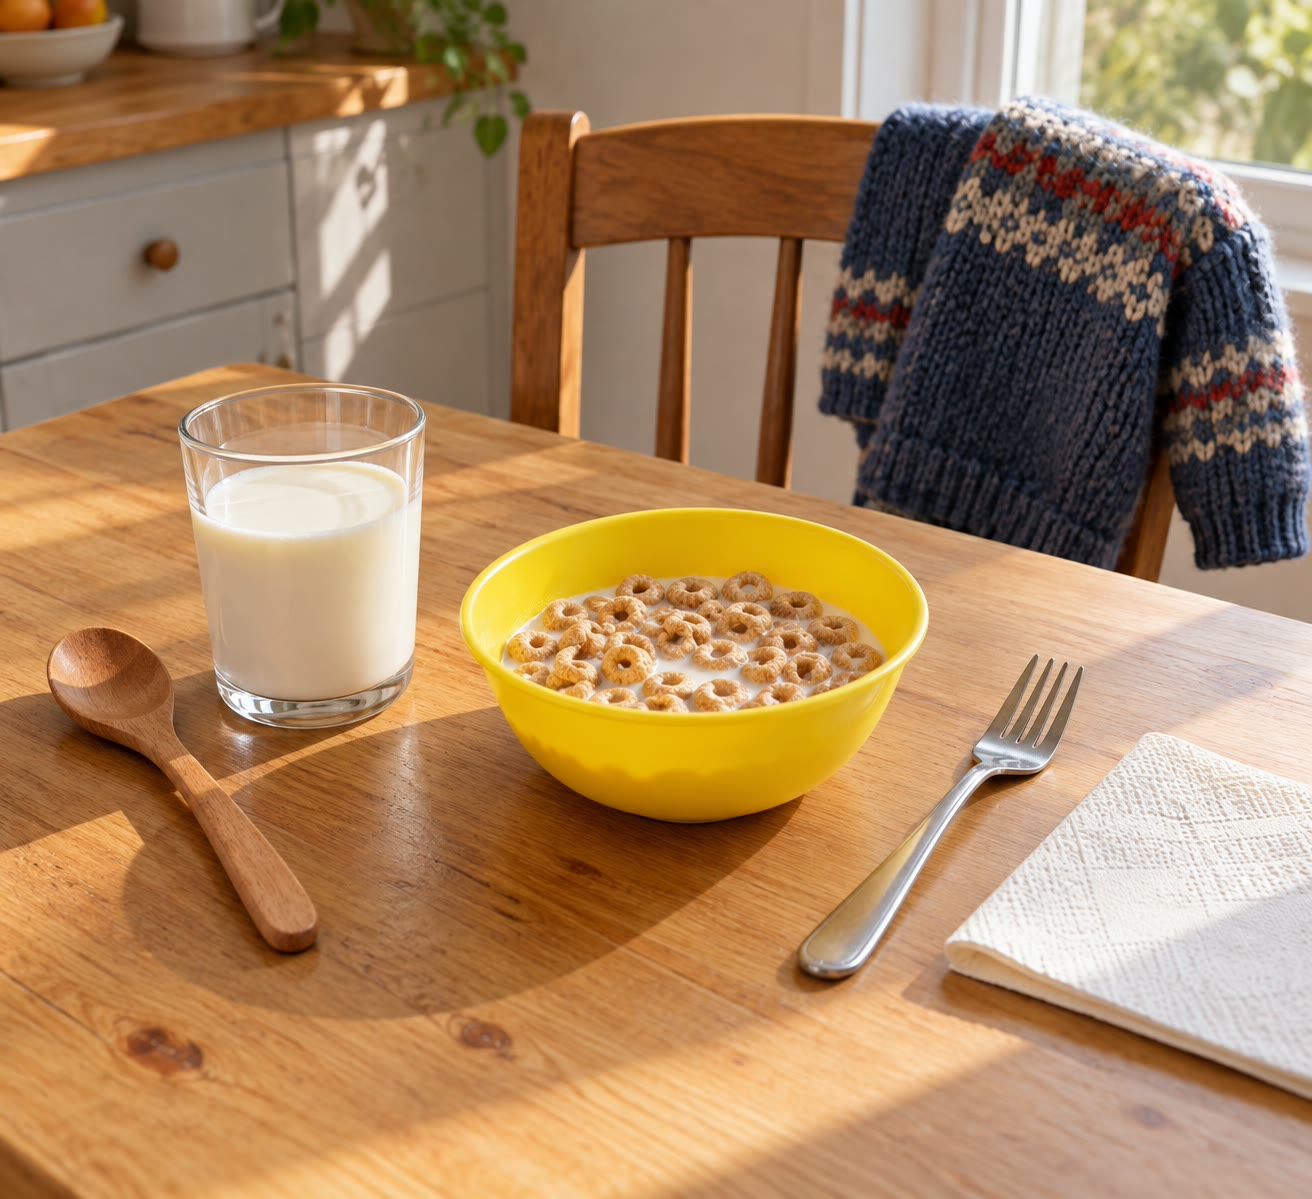
\includegraphics[width=0.62\linewidth]{images/book1/ai/g1-breakfast-table.jpg}

{\small Een ontbijttafel: veel \omterm{def:g1:materials-around-us:object}{voorwerpen}, gemaakt van een paar materialen.}
\end{omfigure}

\section{Voorwerpen en materialen}

\begin{definition}[Voorwerp]\label{def:g1:materials-around-us:object}
Een \emph{voorwerp}\index{voorwerp} is een ding dat we kunnen zien en
aanraken, en dat we vaak kunnen vasthouden en gebruiken: een lepel, een
stoel, een bal, een raam, een schoen.
\end{definition}

\begin{definition}[Materiaal]\label{def:g1:materials-around-us:material}
Het \emph{materiaal}\index{materiaal} van een \omterm{def:g1:materials-around-us:object}{voorwerp} is waar het
\omterm{def:g1:materials-around-us:object}{voorwerp} van gemaakt is. Een lepel kan van hout, van metaal of van
plastic zijn: de lepel is het \omterm{def:g1:materials-around-us:object}{voorwerp}, het hout is het materiaal.
\end{definition}

\begin{example}[Eén voorwerp, drie materialen]\label{ex:g1:materials-around-us:spoons}
Drie lepels liggen naast elkaar. Ze hebben dezelfde vorm en doen
hetzelfde werk, dus zijn het dezelfde soort \omterm{def:g1:materials-around-us:object}{voorwerpen}. Maar de ene is
van hout, de andere van metaal en de derde van plastic: drie
verschillende materialen.
\end{example}

\begin{omfigure}
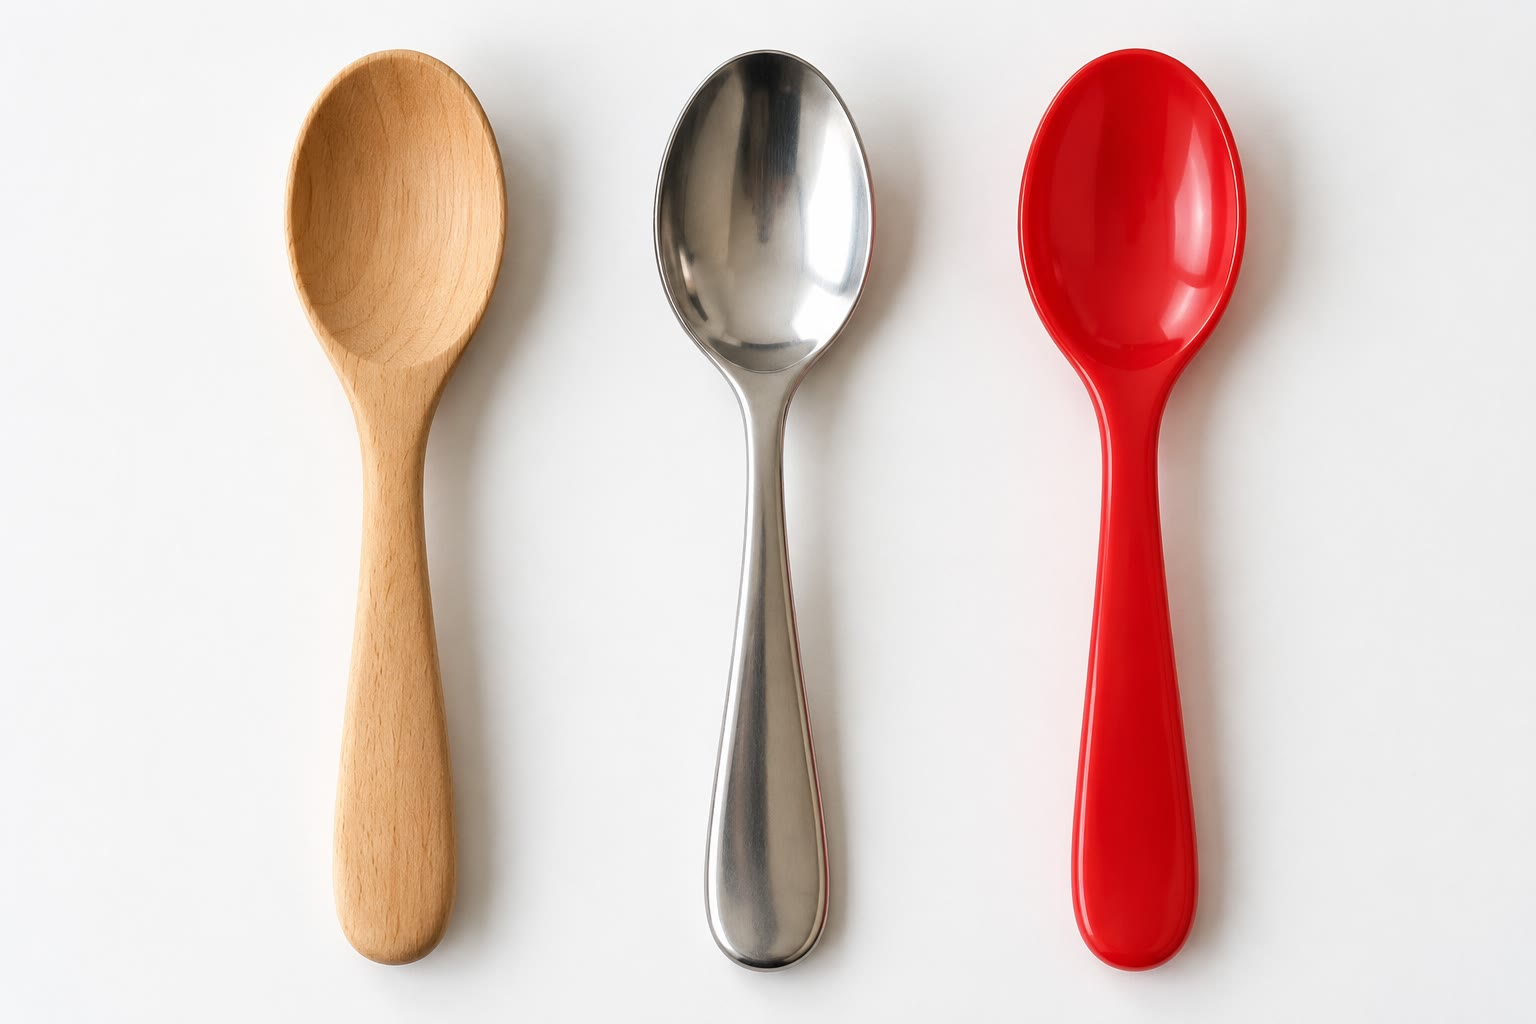
\includegraphics[width=0.55\linewidth]{images/book1/ai/g1-three-spoons.jpg}

{\small Drie lepels: hetzelfde \omterm{def:g1:materials-around-us:object}{voorwerp}, drie materialen --- hout, metaal
en plastic.}
\end{omfigure}

\begin{example}[Eén materiaal, veel voorwerpen]\label{ex:g1:materials-around-us:wood}
Hout is het \omterm{def:g1:materials-around-us:material}{materiaal} van een potlood, een stoel, een deur, een
speelgoedtrein en een houten lepel. Veel verschillende \omterm{def:g1:materials-around-us:object}{voorwerpen} kunnen
van hetzelfde \omterm{def:g1:materials-around-us:material}{materiaal} gemaakt zijn.
\end{example}

\begin{remark}[Voorwerpen uit meerdere materialen]\label{rem:g1:materials-around-us:several}
Veel \omterm{def:g1:materials-around-us:object}{voorwerpen} zijn van meer dan één \omterm{def:g1:materials-around-us:material}{materiaal} gemaakt. Een schaar heeft
bladen van metaal en handvatten van plastic. Een potlood is vanbuiten
hout en vanbinnen een grijs staafje grafiet. Een raam is glas in een
kozijn van hout, metaal of plastic.
\end{remark}

\section{Zeven gewone materialen}

\begin{proposition}[Overal om ons heen materialen]\label{prop:g1:materials-around-us:seven}
De meeste \omterm{def:g1:materials-around-us:object}{voorwerpen} om ons heen zijn gemaakt van een paar gewone
materialen:
\begin{itemize}
  \item \textbf{hout}: tafels, stoelen, potloden, deuren;
  \item \textbf{metaal}: vorken, sleutels, spijkers, pannen, fietsen;
  \item \textbf{glas}: ramen, potten, flessen, drinkglazen;
  \item \textbf{plastic}: kommen, flessen, speelgoed, emmers;
  \item \textbf{papier} en karton: boeken, servetten, dozen;
  \item \textbf{textiel}: kleren, gordijnen, tassen --- gemaakt van wol,
        katoen of andere draden;
  \item \textbf{steen}: muren, traptreden, kiezels, beelden.
\end{itemize}
\end{proposition}

\begin{omfigure}
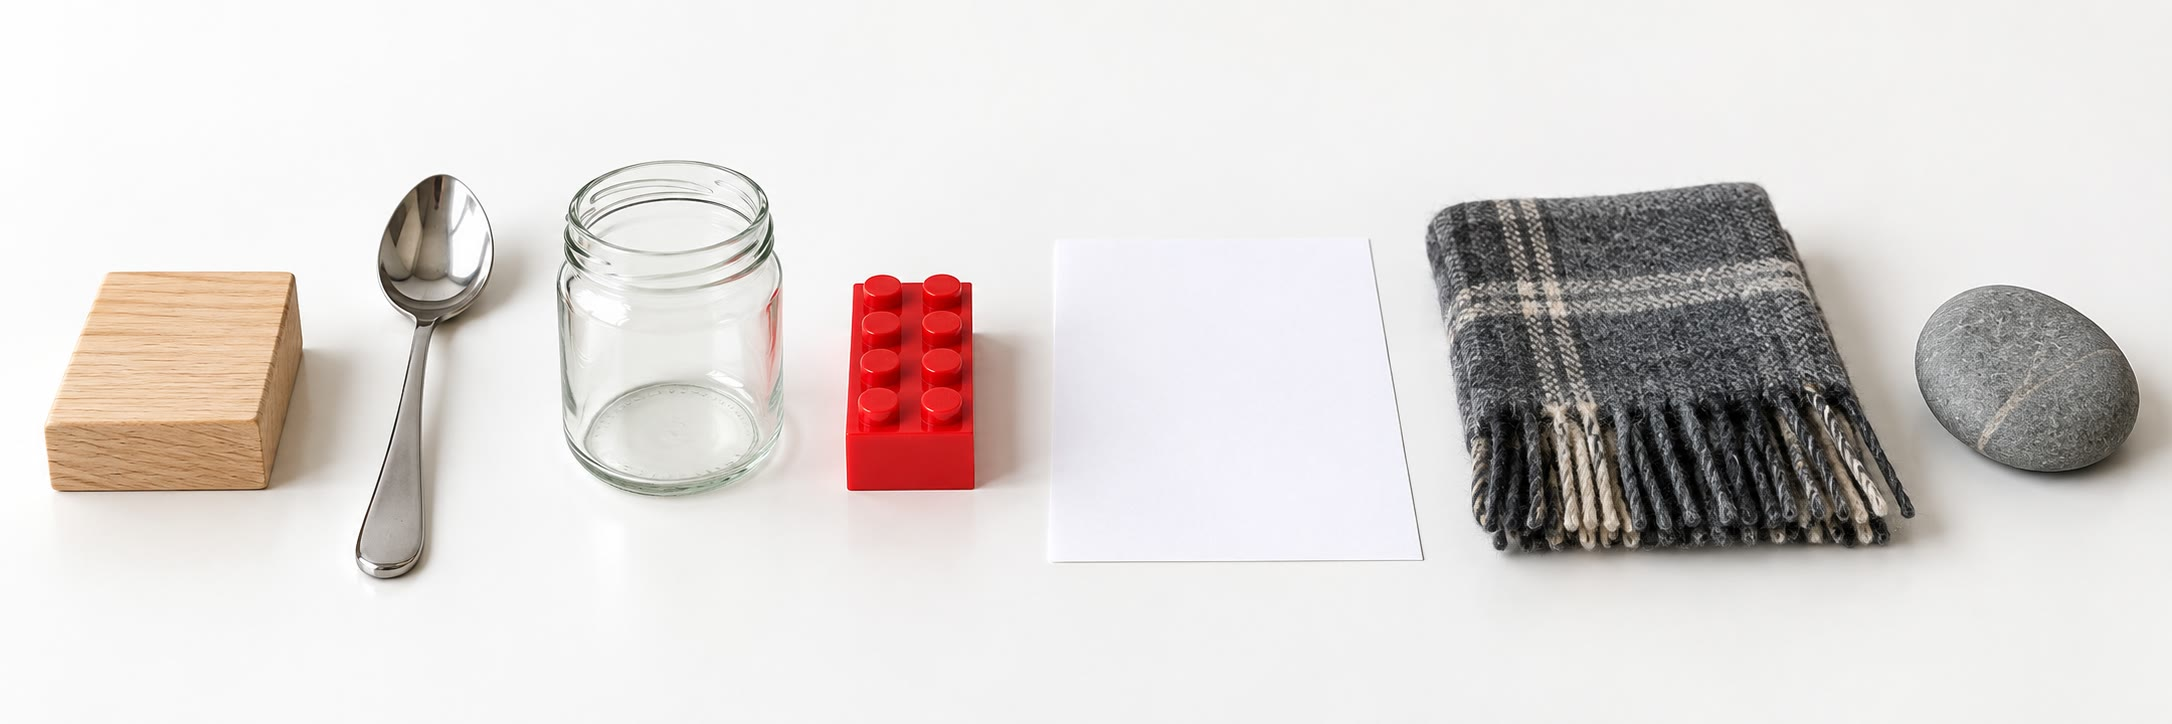
\includegraphics[width=0.75\linewidth]{images/book1/ai/g1-material-samples.jpg}

{\small Zeven stukjes, van links naar rechts: hout, metaal, glas, plastic,
papier, textiel (wol) en steen.}
\end{omfigure}

\begin{remark}[Namen die ook materialen zijn]\label{rem:g1:materials-around-us:names}
We noemen een drinkglas ``een glas'' omdat het van glas gemaakt is, en
een vel papier noemen we soms gewoon ``een papiertje''. Het woord voor
het \omterm{def:g1:materials-around-us:object}{voorwerp} en het woord voor het \omterm{def:g1:materials-around-us:material}{materiaal} zijn dan (bijna) hetzelfde.
Als we het over materialen hebben, bedoelen we de stof, niet het
\omterm{def:g1:materials-around-us:object}{voorwerp}.
\end{remark}

\section{Eigenschappen van materialen}

\begin{definition}[Eigenschap van een materiaal]\label{def:g1:materials-around-us:property}
Een \emph{eigenschap van een materiaal}\index{eigenschap van een materiaal} is
iets wat we erover te weten kunnen komen door te kijken, te voelen of te
testen: is het hard of zacht? Kunnen we erdoorheen kijken? Trekt een
magneet het aan? Blijft het op water drijven of zinkt het?
\end{definition}

\begin{example}[Hard en zacht]\label{ex:g1:materials-around-us:hard}
Een kiezel is hard: als je er met je duim op drukt, blijft er geen deukje
achter. Een wollen sjaal is zacht: hij buigt en vouwt in je hand. Hout,
metaal, glas en steen zijn hard; textiel en papier zijn zacht en buigen
makkelijk.
\end{example}

\begin{example}[Erdoorheen kijken]\label{ex:g1:materials-around-us:see-through}
Door een raam zien we de tuin: glas laat licht door, we zeggen dat het
\emph{doorzichtig} is. Door een houten deur, een bakstenen muur of een
metalen pan kunnen we niet kijken. Sommige soorten plastic zijn
doorzichtig, zoals een waterfles; andere niet, zoals een rood
speelgoedblokje.
\end{example}

\begin{example}[Aangetrokken door een magneet]\label{ex:g1:materials-around-us:magnet}
Een magneet trekt een stalen paperclip, een stalen spijker of een
ijzeren sleutel naar zich toe. Hout, glas, plastic, papier, textiel en steen
trekt hij niet aan. En, gek genoeg, ook niet elk metaal: een blikje van
aluminium en een koperdraad blijven gewoon liggen. Een magneet trekt
\omterm{def:g1:materials-around-us:object}{voorwerpen} van ijzer aan, en van staal, dat vooral uit ijzer bestaat.
\end{example}

\begin{omfigure}
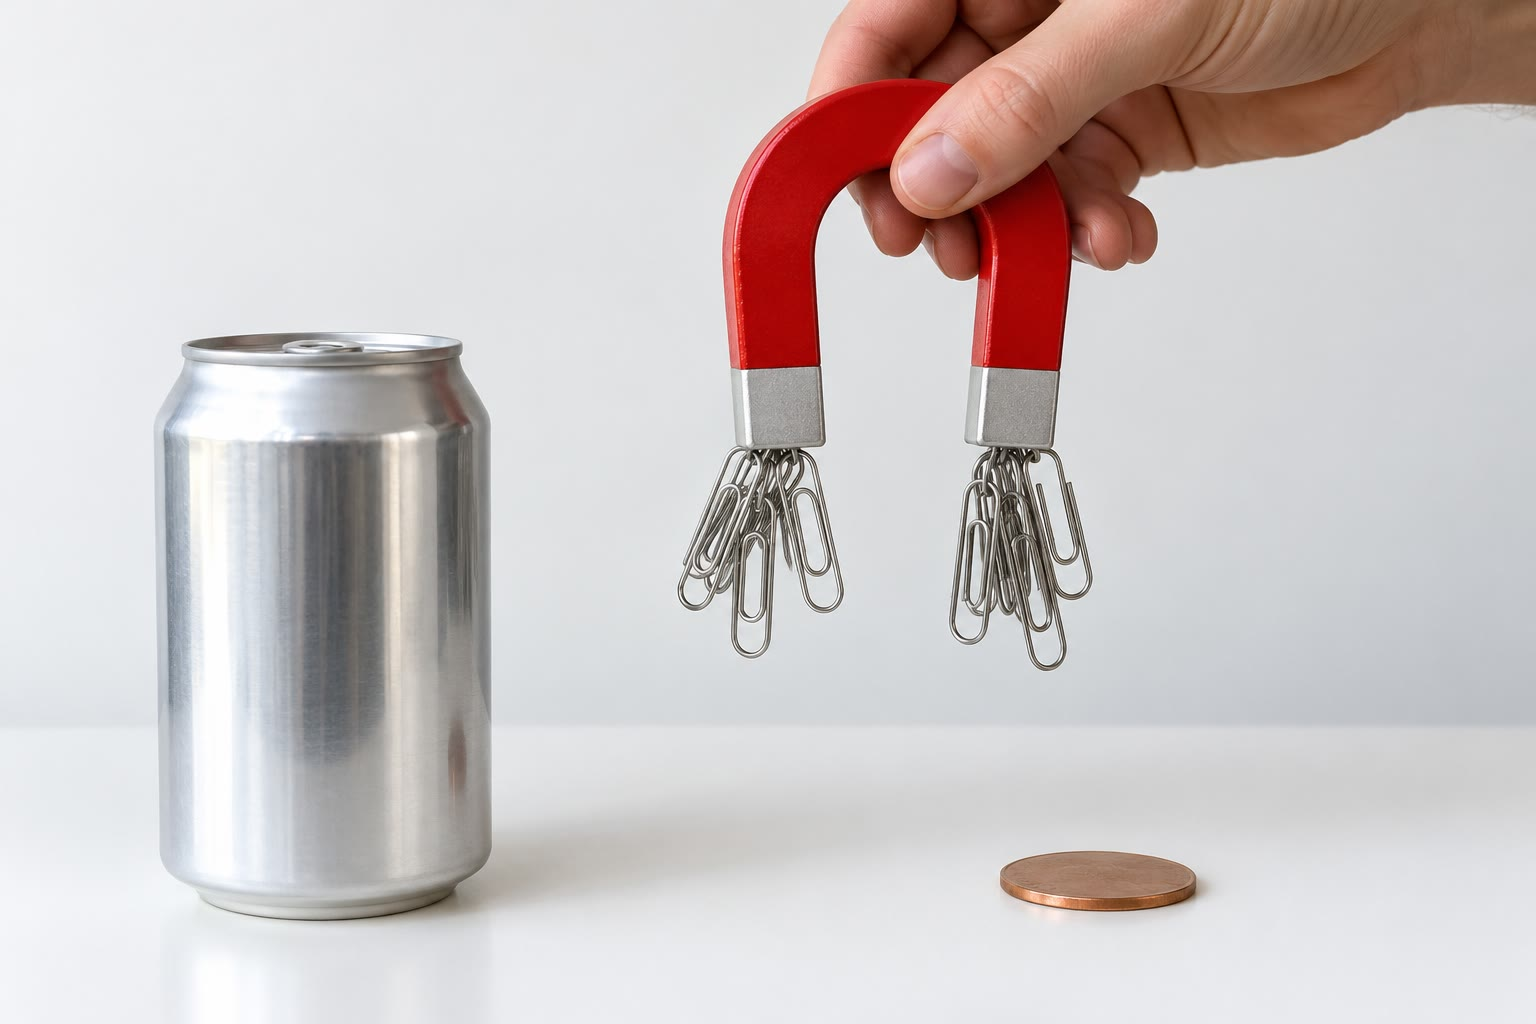
\includegraphics[width=0.55\linewidth]{images/book1/ai/g1-magnet-clips.jpg}

{\small Een magneet tilt stalen paperclips op. Het aluminium blikje en
het koperen schijfje op tafel blijven liggen.}
\end{omfigure}

\begin{example}[Drijven en zinken]\label{ex:g1:materials-around-us:float}
Leg een paar \omterm{def:g1:materials-around-us:object}{voorwerpen} in een bak water. Een houten blokje en een
plastic dop drijven. Een kiezel, een glazen knikker en een stalen
spijker zinken naar de bodem. Of iets drijft of zinkt, is ook een
eigenschap van zijn \omterm{def:g1:materials-around-us:material}{materiaal}.
\end{example}

\begin{omfigure}
\begin{tikzpicture}[font=\small]
  % the basin
  \fill[omWater!80] (0,0) rectangle (9,2.2);
  \draw[omGlass, line width=0.8pt] (-0.1,2.7) -- (0,2.6) -- (0,0) -- (9,0)
    -- (9,2.6) -- (9.1,2.7);
  % floating: wooden block, plastic cap
  \fill[brown!55, draw=brown!70!black] (0.8,2.0) rectangle (2.2,2.5);
  \fill[red!70, draw=red!50!black] (3.7,2.05) rectangle (4.3,2.35);
  % sunk: pebble, marble, nail
  \fill[black!35, draw=black!60] (5.0,0.25) ellipse (0.45 and 0.22);
  \shade[ball color=cyan!40] (6.5,0.2) circle (0.18);
  \fill[black!55] (7.6,0.06) rectangle (8.6,0.14);
  \fill[black!55] (7.52,0.02) rectangle (7.62,0.18);
  % labels
  \node[anchor=south] at (1.5,2.75) {houten blokje};
  \node[anchor=south] at (4.0,2.75) {plastic dop};
  \node[anchor=north] at (5.0,-0.1) {kiezel};
  \node[anchor=north] at (6.5,-0.1) {knikker};
  \node[anchor=north] at (8.1,-0.1) {spijker};
  \node[anchor=west, align=left] at (9.3,2.2) {deze drijven};
  \node[anchor=west, align=left] at (9.3,0.2) {deze zinken};
\end{tikzpicture}

{\small In een bak water: het houten blokje en de plastic dop drijven; de
kiezel, de glazen knikker en de stalen spijker zinken.}
\end{omfigure}

\section{Materialen sorteren}

\begin{method}[Sorteren op één eigenschap]\label{met:g1:materials-around-us:sort}
Zo sorteer je een stapel \omterm{def:g1:materials-around-us:object}{voorwerpen}:
\begin{enumerate}
  \item kies \textbf{één} vraag, bijvoorbeeld ``Trekt een magneet het
        aan?'';
  \item test elk \omterm{def:g1:materials-around-us:object}{voorwerp} en leg het bij de groep ``ja'' of bij de groep
        ``nee'';
  \item sorteer daarna, als je wilt, elke groep nog eens met een andere
        vraag.
\end{enumerate}
Eén vraag tegelijk: zo heeft elk \omterm{def:g1:materials-around-us:object}{voorwerp} precies één plaats.
\end{method}

\begin{omfigure}
\begin{tikzpicture}[font=\small]
  \draw[omDef, line width=1pt] (0,0) circle (2.3);
  \draw[omProp, line width=1pt] (2.4,0) circle (2.3);
  \node[omDef, font=\small\bfseries] at (-0.6,2.65) {van metaal};
  \node[omProp, font=\small\bfseries] at (3.0,2.65) {magneet trekt aan};
  \node[font=\footnotesize] at (-1.1,0.35) {blikje};
  \node[font=\footnotesize] at (-1.1,-0.35) {koperdraad};
  \node[font=\footnotesize] at (1.2,0.6) {stalen spijker};
  \node[font=\footnotesize] at (1.2,0) {ijzeren sleutel};
  \node[font=\footnotesize] at (1.2,-0.6) {paperclip};
  \node[font=\footnotesize] at (3.5,0) {(niets)};
  \node[anchor=west] at (5.2,0.9) {houten lepel};
  \node[anchor=west] at (5.2,0.3) {glazen knikker};
  \node[anchor=west] at (5.2,-0.3) {wollen sjaal};
  \node[anchor=west] at (5.2,-0.9) {kiezel};
\end{tikzpicture}

{\small Twee vragen, twee hoepels. In de blauwe hoepel: de \omterm{def:g1:materials-around-us:object}{voorwerpen} van
metaal. In de oranje hoepel: de \omterm{def:g1:materials-around-us:object}{voorwerpen} die een magneet aantrekt. In
allebei de hoepels: de \omterm{def:g1:materials-around-us:object}{voorwerpen} van ijzer of staal. Buiten allebei:
al het andere.}
\end{omfigure}

\begin{center}
\small
\begin{tabular}{lccc}
\hline
\omterm{def:g1:materials-around-us:object}{voorwerp} (\omterm{def:g1:materials-around-us:material}{materiaal}) & hard? & doorzichtig? & door een magneet aangetrokken? \\
\hline
blokje (hout) & ja & nee & nee \\
spijker (staal) & ja & nee & ja \\
knikker (glas) & ja & ja & nee \\
flessendop (plastic) & ja & nee & nee \\
vel (papier) & nee & nee & nee \\
sjaal (wol) & nee & nee & nee \\
kiezel (steen) & ja & nee & nee \\
\hline
\end{tabular}
\end{center}

\section{Het juiste materiaal voor het werk}

\begin{proposition}[Elk materiaal wordt gekozen om zijn eigenschappen]\label{prop:g1:materials-around-us:choose}
Mensen kiezen het \omterm{def:g1:materials-around-us:material}{materiaal} van een \omterm{def:g1:materials-around-us:object}{voorwerp} naar wat het \omterm{def:g1:materials-around-us:object}{voorwerp} moet
doen:
\begin{itemize}
  \item een raam moet licht binnenlaten: het is van glas, en glas is
        doorzichtig;
  \item een regenjas moet de regen tegenhouden en opgevouwen kunnen
        worden: hij is van plastic of van textiel waar geen water door
        kan;
  \item een pan mag op het fornuis niet smelten: hij is van metaal;
  \item het handvat van een pan mag je hand niet branden: het is vaak van
        hout of van hard plastic, die minder heet worden dan metaal;
  \item een kussen moet zacht zijn: het is van textiel, gevuld met veren of
        vezels.
\end{itemize}
\end{proposition}

\begin{example}[Een bootje]\label{ex:g1:materials-around-us:boat}
Een speelgoedbootje moet drijven. Het kan van hout of van plastic zijn.
Een bootje uit één massief blok steen zou meteen zinken.
\end{example}

\begin{remark}[Gebroken glas]\label{rem:g1:materials-around-us:glass}
Glas is hard, maar het breekt, en de scherven zijn scherp. Als er een
glas breekt, ruimt een volwassene de scherven op.
\end{remark}

\section{Oefeningen}

\begin{exercise}[$\star$]\label{exo:g1:materials-around-us:1}
Is een stoel een \omterm{def:g1:materials-around-us:object}{voorwerp} of een \omterm{def:g1:materials-around-us:material}{materiaal}? Is hout een \omterm{def:g1:materials-around-us:object}{voorwerp} of een
\omterm{def:g1:materials-around-us:material}{materiaal}?
\end{exercise}

\begin{exercise}[$\star$]\label{exo:g1:materials-around-us:2}
Noem het \omterm{def:g1:materials-around-us:material}{materiaal} van elk \omterm{def:g1:materials-around-us:object}{voorwerp}: een ruit, een spijker, een kiezel,
een boek, een sok.
\end{exercise}

\begin{exercise}[$\star$]\label{exo:g1:materials-around-us:3}
Noem twee \omterm{def:g1:materials-around-us:object}{voorwerpen} van hout en twee \omterm{def:g1:materials-around-us:object}{voorwerpen} van plastic.
\end{exercise}

\begin{exercise}[$\star$]\label{exo:g1:materials-around-us:4}
Welke hoort er niet bij, en waarom? Een houten lepel, een metalen vork,
een plastic lepel, een houten stoel. (Kijk naar de materialen.)
\end{exercise}

\begin{exercise}[$\star$]\label{exo:g1:materials-around-us:5}
Door welk \omterm{def:g1:materials-around-us:material}{materiaal} kunnen we kijken: hout, glas of steen?
\end{exercise}

\begin{exercise}[$\star$]\label{exo:g1:materials-around-us:6}
Iemand houdt een magneet bij een stalen spijker, een glazen knikker en
een houten blokje. Welk \omterm{def:g1:materials-around-us:object}{voorwerp} trekt hij aan?
\end{exercise}

\begin{exercise}[$\star$]\label{exo:g1:materials-around-us:7}
Kijk naar de figuur met de bak water. Hoeveel \omterm{def:g1:materials-around-us:object}{voorwerpen} drijven er?
Hoeveel zinken er?
\end{exercise}

\begin{exercise}[$\star$]\label{exo:g1:materials-around-us:8}
Een schaar heeft bladen en handvatten. Van welk \omterm{def:g1:materials-around-us:material}{materiaal} is elk deel
gemaakt? Is een schaar van één \omterm{def:g1:materials-around-us:material}{materiaal} of van twee?
\end{exercise}

\begin{exercise}[$\star$]\label{exo:g1:materials-around-us:9}
Kijk naar de figuur met de twee hoepels. In welke hoepel ligt het
blikje? Waarom ligt het niet in de oranje hoepel?
\end{exercise}

\begin{exercise}[$\star\star$]\label{exo:g1:materials-around-us:10}
Waarom zijn ramen van glas en niet van hout?
\end{exercise}

\begin{exercise}[$\star\star$]\label{exo:g1:materials-around-us:11}
Sam wil deze 8 \omterm{def:g1:materials-around-us:object}{voorwerpen} sorteren met de vraag ``Trekt een magneet het
aan?'': een stalen spijker, een paperclip, een kiezel, een houten lepel,
een ijzeren sleutel, een blikje, een glazen knikker, een wollen sok.
Hoeveel \omterm{def:g1:materials-around-us:object}{voorwerpen} komen in de groep ``ja''? Hoeveel in de groep
``nee''?
\end{exercise}
